% !TEX root = ../main.tex

\chapter{Implementation}

This chapter outlines and covers the process of implementation of the project. This includes the technologies used for the project, as well as the breakdown of the structure and implementation of the different parts of the project.

\section{Technology Used}

There are various technologies used within this project. These are Python 3.9, Visual Studio Code, Git and Github, Command-Line Interface, AntConc 3.5.9, Rocksteady 0.4 and Gretl. Each of these had a different function within the project.

\subsection{Python 3.9}

Python is an interpreted, high-level and general-purpose programming language. The version used was version 3.9. 

Python was used in this project to develop and execute the procedures outlined in the implementation. This is due to the fact that python is a very useful language for handling projects which require a large amount of various different features as it is general purpose. For that reasons it has many publicly available libraries which help for many of the scenarios come across throughout development.

The libraries used had three main purposes: file handling, data tidying and mathematical operations.

\subsubsection{File Handling}

In order to handle the files downloaded from \emph{lexisnexis} and \emph{proquest}, various libraries and modules had to be used. The libraries and modules being \verb|sys|, \verb|os| and \verb|striprtf|.

The \verb|sys| module provides functions and variables used to manipulate different parts of the Python runtime environment. It is used to create a global variable which allowed the setting of a source for files, and allowed this to be used throughout the various files in the program. The source being the choice between using \emph{lexisnexis} and \emph{proquest} files.

The \verb|os| module provides functions and variables used to perform operating system tasks. It is used to access environment variables, as well as to help parse through files in a given directory.

The \verb|striprtf| library is used to translate rtf to a python string. When files are downloaded from \emph{lexinexis} they are in rtf format. This library is used to help parsed the information in these files into a usable format.

\subsubsection{Data Tidying}

In order to tidy up the data extracted from articles and make it usable in the context required the use of some libraries is needed. These libraries and modules are \verb|pandas|, \verb|json|, \verb|copy|, \verb|datetime|, \verb|operator|, \verb|matplotlib|, \verb|seaborn| and \verb|warnings|.

The \verb|pandas| is an open source data analysis and manipulation tool. This library is used to aid in the tabling of data. This was useful in order to use this data within graphs and to create an excel spreadsheet. For graphing timeseries, this library was especially useful with it's \verb|to_datetime()| function which allowed the dates to be appropriately used as indices. This is significant especially when comparing two separate time series, as it spaced the values according to date and not which datapoint it is along the sequence.

The \verb|json| library is used to dump json data from files and the extract it back from the file in order to cache the information extracted for future use.

The \verb|copy| library is used to create deepcopies of json objects. This is necessary as the copies had to be completely separate from the original version, and due to how python works this cannot simply be done through a shallow copy. Therefore the library was used to facilitate this.

The \verb|datetime| module supplies classes for manipulating dates and times. As they are usually stored in strings they can be complex to perform operations with. The library makes this process a lot more straightforward.

The \verb|operator| module exports a set of efficient functions corresponding to the intrinsic operators of Python. It is used sort arrays of json objects that contain a given key. This was very useful when ordering data entries by date.

The \verb|matplotlib| library provides an object-oriented API for embedding plots into applications using general-purpose GUI toolkits like Tkinter, wxPython, Qt, or GTK. It therefore aids in the creation and display of graphs within the system.

The \verb|seaborn| library is a data visualization library based on matplotlib. It helps the graphs look more aesthetically pleasing as well helping them become cleaere, therefore easier to read.

The \verb|warnings| module is used in order to supress warnings. This helps make the program be easier to read for an end user.

\subsubsection{Mathematical Operations}

In order to perform mathematical operations appropriately multiple libraries are used. This is to avoid the recreation of tested and efficient functions, and avoid any potential errors when recreating them. These libraries and modules are \verb|numpy|, \verb|statistics|, \verb|scipy|, \verb|math|, \verb|sklearn| and \verb|time|.

The \verb|numpy| is a Python library used for working with arrays. It also has functions for working in domain of linear algebra, fourier transform, and matrices.

The \verb|statistics| is a built-in Python library for descriptive statistics.

The \verb|scipy| is a collection of mathematical algorithms and convenience functions built on the \verb|numpy| extension of Python. It adds significant power to the interactive Python session by providing the user with high-level commands and classes for manipulating and visualizing data. Specifically the \verb|scipy.stats| module was used. Similarly, to the \verb|statistics| library it was used to gather various types of statistical information.

The \verb|math| module is a built-in module that you can use for mathematical tasks. It is used specifically for the \verb|log()| function contained within.

The \verb|sklearn| library is an incredibly useful machine learning library. The \verb|sklearn| library contains a lot of efficient tools for machine learning and statistical modeling including classification, regression, clustering and dimensionality reduction. It is used for the machine learning functionality required for the \verb|singlePointEstimator|. These being various trainable models, appropriately metric measuring functions, and some utility functions.

The \verb|time| module provides various time-related functions. Most of the functions defined in this module call platform C library functions with the same name. This important because it is used to time some elements of the system, and these timings must be precise.

\subsection{Visual Studio Code}

Visual Studio Code is a freeware source-code editor made by Microsoft for Windows, Linux and macOS. Features include support for debugging, syntax highlighting, intelligent code completion, snippets, code refactoring, and embedded Git. It was used to ease the development of the codebase.

\subsection{Git and Github}

Git is a version control system. Git tracks the changes you make to files, so you have a record of what has been done, and you can revert to specific versions should you ever need to. Git allows changes by multiple people to all be merged into one source. This can be used to create features then once they are complete merge them into a final version of the system.

GitHub is a provider of Internet hosting for software development and version control using Git. It offers the distributed version control and source code management functionality of Git, plus its own features.

\subsection{Command-Line Interface}

A command-line interface processes commands to a computer program in the form of lines of text. It is used to execute the programs developed, git commands and any other required commands.

\subsection{AntConc 3.5.9}

AntConc is a freeware corpus analysis toolkit for concordancing and text analysis. It is used for preliminary text analysis of the articles downloaded from \emph{lexisnexis} and \emph{proquest}. It can be used to create words lists, n-grams, concordance plots, amongst other useful tools that may be used to examine word choices in texts.

\subsection{Rocksteady 0.4}

Rocksteady is a sentiment analysis tool. It creates a timeline of sentiment, and allows the filtering as well as visualisation of this data. It is used within this project to understand how the sentiment proxy extraction process works.

\subsection{Gretl}

Gretl is an open-source statistical package, mainly for econometrics. The name is an acronym for Gnu Regression, Econometrics and Time-series Library. It has both a graphical user interface and a command-line interface. It was mainly used for vector autoregression within this project.

\section{Setting up the System}

The technologies that have been used to implement the system have been covered. This section therefore covers the details of the implementation of the indivdual components laid out in the design, using these technologies.

The system is run as a script using the terminal. The commmand for initiating the program being \verb|python IntelligentAnalysis.py|. This is assuming that the default version of python running is version 3.9, otherwise the command may have to be modified slightly to accomodate for this. The full codebase can be found at the following url: \url{https://github.com/DaVinciTachyon/FinalYearProject}. This command is run from the root directory of this git repository.

\subsection{The Price Gatherer}

The Price Gatherer has a straightforward flow. Thus making the understanding of it's implementation quite simple.

\subsubsection{The Price Source}

The Price Source component has one main function. That is to contact the IEX Cloud API and return the past 5 years of price points for a given stock.

This component does require a bit of set up in order to have access to the api:
\begin{enumerate}
    \item Register for IEX Cloud
    \item Gain access to and retrieve an API key
    \item Insert API key into environment variables
\end{enumerate}

Once these steps are done the component itself can be used. The component can be divided into a few different steps:
\begin{enumerate}
    \item Check if the cache exists
    \begin{itemize}
        \item If cache exists, load items from cache
        \item otherwise, continue
    \end{itemize}
    \item Load API key from environment
    \item Create API request, with certain important information:
    \begin{itemize}
        \item URL -- This contains the API Key and Stock Symbol
        \item API Key
        \item Stock Symbol
        \item Period desired -- This is set to 5 years given the payment tier chosen on the website
    \end{itemize}
    \item Gather API response into JSON String
    \item Sort the JSON array by date
    \item Cache the data
\end{enumerate}

An important item to highlight within this procedure are the use of a caching system. This allows for a large speed up in the process of gathering prices, when the program is run for a second time. As well as this it save a lot of money in API fees and network access fees. The caching system in this case is the creation of a json file, however, it may be optimised to use a database.

In order to get the cache, the program check whether the file containing th edata exists, if it does it opens the file and loads the data as a json string. It can be seen below:
\begin{lstlisting}[caption=Loading Prices Cache]
if os.path.isfile(pricesFilename):
    with open(pricesFilename) as json_file:
        data = json.load(json_file)
\end{lstlisting}
The cache is the created by opening a file and simple dumping the json string within, as can be seen here:
\begin{lstlisting}[caption=Creation of Prices Cache]
with open(pricesFilename, 'w') as json_file:
    json.dump(data, json_file)
\end{lstlisting}

Another item to not is the sorting of the JSON array. This is usually a more complex process, however, the \verb|operator| module eases this process significantly.
\begin{lstlisting}[caption=Sort JSON Array]
sorted(data, key = operator.itemgetter('date'))
\end{lstlisting}

\subsubsection{Key Filtering}

The key filtering process takes in the full data-set and the keys desired for each element of the data-set. It then creates a new data-set with only the desired keys extracted. This is currently a \verb|for| loop which goes through the entire data-set adding each entry individually.
\begin{lstlisting}[caption=Filtering Desired Keys]
for entry in originalDataset:
    filteredEntry = {}
    for key in keys:
        filteredEntry[key] = entry[key]
    newDataset.append(filteredEntry)
\end{lstlisting}
The current solution has a time complexity of \verb|O(N)|, where N is the length of the data-set. Some research has been done in order to find a more efficient solution, however, so far this has been unsuccessful.

\subsubsection{The Return Adder}

This component requires an array of numbers for the returns to create. What this means the that it will reveceive a 1 in the array if it wants to calculate 21 days returns. It then loops through the data-set adding the appropriate returns to the given entry.

The return cannot be added to the first n days, this is simply done using an \verb|if| statement to make sure to not attempt this before it is possible.

The formula used for return is $log(\frac{r_t}{r_{t - l}})$ where $r$ is the return, $t$ is the current day, and $l$ is the number of days being used.

The final code put this all togther in the following way:
\begin{lstlisting}[caption=Adding Returns]
for t in range(len(prices)):
    for l in returnLengths:
        if(t >= l):
            prices[t][f"return{l}Day"] = math.log(prices[t]['close']/prices[t-l]['close'])
\end{lstlisting}

\subsection{The Sentiment Gatherer}

The Sentiment Gatherer can be divided into three main subsections, each one of those being divided into two components. It is important to not that the first two main subsections can be run in parallel, and must be run before the last. The Article Source and Article PArser compose this first subsection. This can be run in parallel to the Dictionary and Key Filtering components. However, they must all be run before the Sentiment Extractor and consequently the Z-Scores components.

\subsubsection{The Article Source}

The Article Source component has one main function. That is to gather the dowloaded articles and import them into the system.

This component requires a bit of set up:
\begin{enumerate}
    \item Log into LexisNexis with Trinity credentials
    \item Search for a given company
    \item Download articles, this part has a few steps:
    \begin{enumerate}
        \item Select rtf format
        \item Remove formatting from files
        \item Download 500 files by giving an appropriate range -- this is the maximum available for downloading at once
        \item Repeat from step (a) 5 times
    \end{enumerate}
    \item Wait 2 hours -- Once 5 downloads have been executed, LexisNexis does not allow any more dowloads for 2 hours
    \item Repeat from step 1 as many times as necessary
\end{enumerate}
Using this process 7000 articles were dowloaded for this iteration of the system, for the given company, which will be discussed later on. The reason for the choice of 7000 article is due to the fact that they cover the 5 year range covered by the Price Source quite thoroughly. They are a significant amount of articles, however more could be dowloaded. That said they covered the requirements for this project.

There was though of automating this procedure in order to improve up this process. This would expedite the process and lead to the ability to download a lot more articles. There were a few reasons this was not done:
\begin{itemize}
    \item The 2 hour wait is still required, therefore the process would not be expedited significantly
    \item The amount of articles gathered manually were sufficent for this project
    \item There was a focus on creating other parts of this project, as the creation of this automation would require a significant amount of time
\end{itemize}

Once these step are executed and the downloaded files are placed in the correct directory the component functionality is complete.

\subsubsection{The Article Parser}

The Article Parser Component gathers the articles and turns them into a format usable by the system. The component can be broken down similarly to the Price Source component with some differences:
\begin{enumerate}
    \item Check if the cache exists
    \begin{itemize}
        \item If cache exists, load items from cache
        \item otherwise, continue
    \end{itemize}
    \item Find all files with articles
    \item Iterate through all the files, doing the following:
    \begin{enumerate}
        \item Read the contents of the file and assign them to an rich text format (rtf) string
        \item Parse the rtf string into a legible string using the \verb|rtf_to_text()| function
        \item Split the string into the articles contained
        \item Parse the article strings into a JSON object containing the required content and metadata
        \item Append the articles to a JSON array
    \end{enumerate}
    \item Cache the article JSON array
\end{enumerate}

The caching system is identical to the Price Source, the JSON array is dumped to a file and extracted from the file when required.

The extraction of the articles from the file into an rtf string has a point that should be highlighted. The way this works requires each line to be extracted separately, then concatenated to the previous, until the full file is extracted. This part of the program was given in order to aid in the project, however it was quite inefficient. The original code looked like this:
\begin{lstlisting}[caption=Slow Text Extraction]
fileContent = ''
for line in file:
    if line.strip() != '':
        fileContent += line + "\n"
    else:
        fileContent += line
\end{lstlisting}
The improvement made to the code then looked like this:
\begin{lstlisting}[caption=Optimised Text Extraction]
fileContent = "".join([f"{line}\n" if line.strip() != '' else f"{line}" for line in file])
\end{lstlisting}
Beyond reducing the number of lines in the program and looking cleaner, this change creates a radical change in the speed of the program. The program was run on the 7000 articles, and originally was let run for 12 hours before being terminated. Then once the change was made the program consistently finishes within 5 minutes. The reason for this being such a big deal is that if there were more articles added, the entire program would have be run again. The reason for the for the speed difference explains why there is such a large timing difference.

The original way uses the \verb|+=| operator, what this means is that an array is created for the original string, as a string is a character array, then a new character array is created with the new appropriate length in order to allow for the change. This is quite a costly process both timewise and spacewise, and it is repeated for every line in every file. It is important to remember that each time this process is executed the array becomes bigger, making it a slower process each time.

The optimised method used the the \verb|"".join()| function. The way works is that it creates a set of strings one for each line, then does the joining only once. Therefore the large array array has to be created only once and does not have to have its size change.

The final point to discuss is the parsing of the python string into a JSON array. In order to utilise the information in an easier manner, some metadata is extracted alongside the content of the article itself. Each article is represented by a JSON object with the following keys:
\begin{itemize}
    \item \texttt{title} -- The article title
    \item \texttt{source} -- The name of the publication the article was published in
    \item \texttt{date} -- The date the article was published
    \item \texttt{copyright} -- The type of copyright of the article
    \item \texttt{length} -- The length of the body of the article
    \item \texttt{section} -- If the article is divided into parts, this will indicate which part this is
    \item \texttt{language} -- The language the article is in, for this project, the articles are in English
    \item \texttt{pubtype} -- The type of publication the article was published in - newspaper, magazine, etc.
    \item \texttt{subject} -- Key words which describe the article contents
    \item \texttt{geographic} -- The locaiton of publication
    \item \texttt{loaddate} -- The date the article was uploaded to the the Article Source
    \item \texttt{byline} -- The author(s) of the article
    \item \texttt{body} -- The contents of the article
\end{itemize}
These metadata items are extracted into the array from the original string by using certain indicators withing the text. An example of such an indicator would be that the line containing the source thatsrts with \verb|"Source:"|. This is executed in the code the following way:
\begin{lstlisting}[caption=Source Extraction]
if tempLine.startswith('Source:') and extractValue(line) != '':
    document['source'] = extractValue(line)
\end{lstlisting}
The \verb|extractValue| function simple removes the indicator, allowing for the extraction of the value only.

The special case is the body. This still has indicators. The indicator of the start of the body is simply a line only containing \verb|"Body"| and the end of it is simple represent by \verb|"End of Document"|. The lines within these two indicatos are simply concatenated with each other and assigned to the correct key at the end. The \verb|+=| operator is used for this. There is room for creation of efficiency, however, due to the relatively short nature of these articles, this is efficient enough for use within this process currently. In the future this would be an area to explore the creation of such efficiencies.

\subsubsection{The Dictionary}

The dictionary is extracted from the Rocksteady files. If there were future development to this project it may be worth spending time adding more entries, as well as making the sentiment choice more specific to the context of the articles that are chosen. An example of such a thing would be that for a company such as Gamestop the word game may have positive sentiment, even though in general it may have no sentiment attached.

The extraction of the entries from the excel file is very simply achieved with the use of the pandas library. The following function extracts all the entries and associates each item to it's correct row and column.
\begin{lstlisting}[caption=Dictionary Extraction]
data = pd.read_excel(r"./dictionaries/inquirerbasic.xls") 
\end{lstlisting}

\subsubsection{Key Filtering}

This process of extracting only the desired sentiment attribute columns is achieved through the use of a dataframe. It takes the data-set from the previous component and an array containing the titles of the desired columns as inputs, and returns only said columns.
\begin{lstlisting}[caption=Key Filtering Dataframe]
df = pd.DataFrame(data, columns= ['Entry', 'Positiv', 'Negativ']).to_numpy()
\end{lstlisting}
The dataframe is then turned into a dictionary object. What this does is it assigns the values of the desired sentiment attribute columns to the word itself. The object will have the following format: \verb|{ word: [ sentimentColumnValue ] }|. This is achieve with the following segment of code:
\begin{lstlisting}[caption=Dictionary Creation]
dictionary = {}
for index, item in enumerate(df):
    dictionary[item[0]] = item[1:]
\end{lstlisting}
It is important to note that \verb|item[0]| is the word itself and the rest of the items in the array are the sentiment attribute column values.

\subsubsection{The Sentiment Extractor}

This component can be broken down into two steps:
\begin{enumerate}
    \item Extraction
    \item Date Joining
\end{enumerate}

\paragraph{Extraction}

This step takes in the articles from the Article Parser and the Dictionary from the Key Filtering. It then creates a new array of JSON Objects. Each object represent an article. Each object has the following keys:
\begin{itemize}
    \item \texttt{date} -- The date key from the article
    \item \texttt{totalWords} -- The length key from the article
    \item \texttt{positiveSentiment} -- The number of words that have the \verb|Positiv| attribute determined by the dictionary
    \item \texttt{negativeSentiment} -- The number of words that have the \verb|Negativ| attribute determined by the dictionary
\end{itemize}
If more sentiment attributes were to be included they would have an extra key assigned to them. The sentiment attribute keys are found by iterating through all the words in the body of the article and tallying the words according to which columns are labeled true in the dictionary.

\paragraph{Date Joining}

This step takes the array created in the previous step and merges all of the elements on any given day together. This means the final JSON object will be an array ordered by date with the following keys:
\begin{itemize}
    \item \texttt{date} -- The date of the articles
    \item \texttt{articles} -- The total number of articles on said day
    \item \texttt{totalWords} -- The total number of words in all the articles
    \item \texttt{positiveSentiment} -- The number of words that have the \verb|Positiv| attribute determined by the dictionary in all the articles
    \item \texttt{negativeSentiment} -- The number of words that have the \verb|Negativ| attribute determined by the dictionary in all the articles
\end{itemize}
Similarly to the Price Gatherer, the array is ordered by date in the following way:
\begin{lstlisting}[caption=JSON Array Ordered by Date]
sentimentByDate = sorted(sentimentByDate, key = operator.itemgetter('date'))
\end{lstlisting}

\subsubsection{Z-Scores}

This component can be divided into four steps:
\begin{enumerate}
    \item Column Separation
    \item Percentage Calculation
    \item Z-Score Calculation
    \item Object Assignment
\end{enumerate}

\paragraph{Column Separation}

The array created in the Sentiment Extractor is iterated through and an array is created for each key within the objects. This means that each key will have its own array.

\paragraph{Percentage Calculation}

In this project it is important to undesrtand relative amounts. Therefore a few different percentages must be calculated. The sentiment columns are replaced with the percentage of sentiment words in relation to the total number of words for that article. The totalWords column is replaced with the percentage of words in relation to the number of articles.

\paragraph{Z-Score Calculation}

The \verb|scipy.stats| module is then used to calculate the z-score for each in element in each of the arrays, excluding the \verb|date| array. An example of this is:
\begin{lstlisting}[caption=Z-Score Calculation]
articles = stats.zscore(articles)
\end{lstlisting}

\paragraph{Object Assignment}

The final step in the component is create an array from the separated array with the following keys:
\begin{itemize}
    \item \texttt{date} -- date of the data-point
    \item \texttt{articles} -- z-score of number of articles
    \item \texttt{totalWords} -- z-score of number of total words
    \item \texttt{positiveSentiment} -- z-score of number of positive sentiment words
    \item \texttt{negativeSentiment} -- z-score of number of negative sentiment words
\end{itemize}
This will still be ordered by date, as the order was never changed.

\subsection{The Analyser}

The Analyser is composed of various unrelated components, which are preceded by three components which allow the other to achieve their tasks efficently, and in an easy to execute manner. The inital three components are the following: 
\begin{itemize}
    \item The User Interface
    \item The Joiner
    \item The Period Selector
\end{itemize}

\subsubsection{The User Interface}

The User Interface is essential towards creating a navigatable environment for users of the system. In a very basic sense it is a set of menus which allows the selection of which tool to use within the Analyser, and selected the desired parameters for these tools.

These menus work by showing a user a set of options, and allowing the user to put in a number in order to select one of these. This methods allows for full usage of the program, and allows limitations to be imposed so that it may not be abused. The steps to achievinng one of the menus is the following:
\begin{enumerate}
    \item Print out the options so that the user may know what they are
    \item Request the input
    \item Ensure the input is an integer, and convert the string input to one
    \item Select the appropriate the appropriate function to run given the option selected, or repeat the question if the input was erroneous
\end{enumerate}

\paragraph{Step 1}

The options can be laid out with the following code:
\begin{lstlisting}[caption=Menu Options]
print("1: 1 year", "2: 2 year", "3: 3 year", "4: maximum available", sep="\t")
\end{lstlisting}

\paragraph{Step 2}

Python has a function to simplify the process of gathering the input. The input has the \verb|strip()| function run on it in order to remove beginning and ending whitespace, just incase this is done by mistake.
\begin{lstlisting}[caption=Get Input]
sampleSize = input("Please select the length of your sample size: ").strip()
\end{lstlisting}

\paragraph{Step 3}

In order to ensure the input is a valid integer the follwing statement is run. It simply checks if the input is a digit, and if it is it converts it to an integer.
\begin{lstlisting}[caption=Check if Integer]
if sampleSize.isdigit():
        sampleSize = int(sampleSize)
\end{lstlisting}

\paragraph{Step 4}

The correct function is selected in one of two methods.
\begin{enumerate}
    \item A set of \verb|if|/\verb|elif| statements, since a \verb|switch-case| statement does not exist in python
    \begin{lstlisting}[caption=If/Elif Statements]
    if section == 1:
        dataset = prices
    elif section == 2:
        dataset = sentiment
    \end{lstlisting}
    \item Check if the input is an integer and in the desired range, and can be given into the function
    \begin{lstlisting}[caption=Integer Range Choice]
    if isinstance(column, int) and column > 0 and column <= len(keys):
        column = keys[column - 1]
    \end{lstlisting}
\end{enumerate}

The \verb|isinstance| function allows the system to determine if a variable is an instance of a given type. In this case if it is an \verb|int|.

Both of the allow for the situation where an input is entered incorrectly. In these cases the \verb|else| option is chosen which asks you to try again, and the boolean which determines whether the item has been chosen is set kept as false, since it is set to true in other cases.

\subsubsection{The Joiner}

The Joiner wants the prices and sentiment data-sets to overlap. This has a requires a few step to be excuted in ored to be achieved:
\begin{enumerate}
    \item Select start date -- this will be the start date of the data-set that starts later between the two
    \item Select end date -- this will be the end date of the data-set that ends earlier between the two
    \item Find the element indexes for start and end dates for both data-sets
    \item Create data-sets with new start and end indexes
    \item Add empty elements to days where the datset does not have a day the other does, in order to have fully overlapping data-sets
\end{enumerate}

For step 4, this can be achieved using the following notation within Python: \verb|prices[priceStart:priceEnd], sentiment[sentStart:sentEnd]|, where the indexes have been previously discovered.

For step 5, the empty objects are the following:
\begin{itemize}
    \item For a day with no sentiment
    \begin{lstlisting}[caption=No Sentiment Day]
    {'date': prices[i]['date'], 'articles': 0, 'totalWords': 0, 'positiveSentiment': 0, 'negativeSentiment': 0}
    \end{lstlisting}
    \item For a day with no price activity
    \begin{lstlisting}[caption=No Price Day]
    {'date': sentiment[i]['date'], 'close': prices[i - 1]['close'], 'symbol': prices[i]['symbol'], 'volume': 0}
    \end{lstlisting}
\end{itemize}

It is important to note that this step is done on the the full values of these arrays, then the z-scores are calculated afterwards.

\subsubsection{The Period Selector}

This item has it's own menu that runs after the tool to use has been selected. It allows the choice between 4 different periods. These being:
\begin{itemize}
    \item 1 year -- The data-sets returned will start 1 year before the end date of the data-sets, and have all the following values
    \item 2 years -- The data-sets returned will start 2 years before the end date of the data-sets, and have all the following values
    \item 3 years -- The data-sets returned will start 3 years before the end date of the data-sets, and have all the following values
    \item maximum available -- The full data-sets will be used
\end{itemize}
This is done by getting the date of the last element, and subtracting the appropriate time from it. The date is an instance of \verb|datetime|, not a string.
\begin{lstlisting}[caption=Subtract years]
date - relativedelta(years=years)    
\end{lstlisting}
All of the elements with a date including and past the start date are then return as the data-set to be used.

\subsubsection{Return Vs Sentiment Grapher}

The menu for this component allows the user to select the prices columns and sentiment columns they which to visualise.

The first step towards creating these graphs is inserting the objects into dataframes, where the indexes are the sets of dates as \verb|datetime| instances. This enables them to be used as timeseries.

The next step is to use the \verb|matplotlib| library in order to create the graphs themselves. The figure on which the graph will be displayed needs to be split into two subplots. These will be overlapping each other, with the x-axis being the date, and the y-axis being on one side representative of the price and the other the sentiment.

\begin{figure}[h]
    \centering
    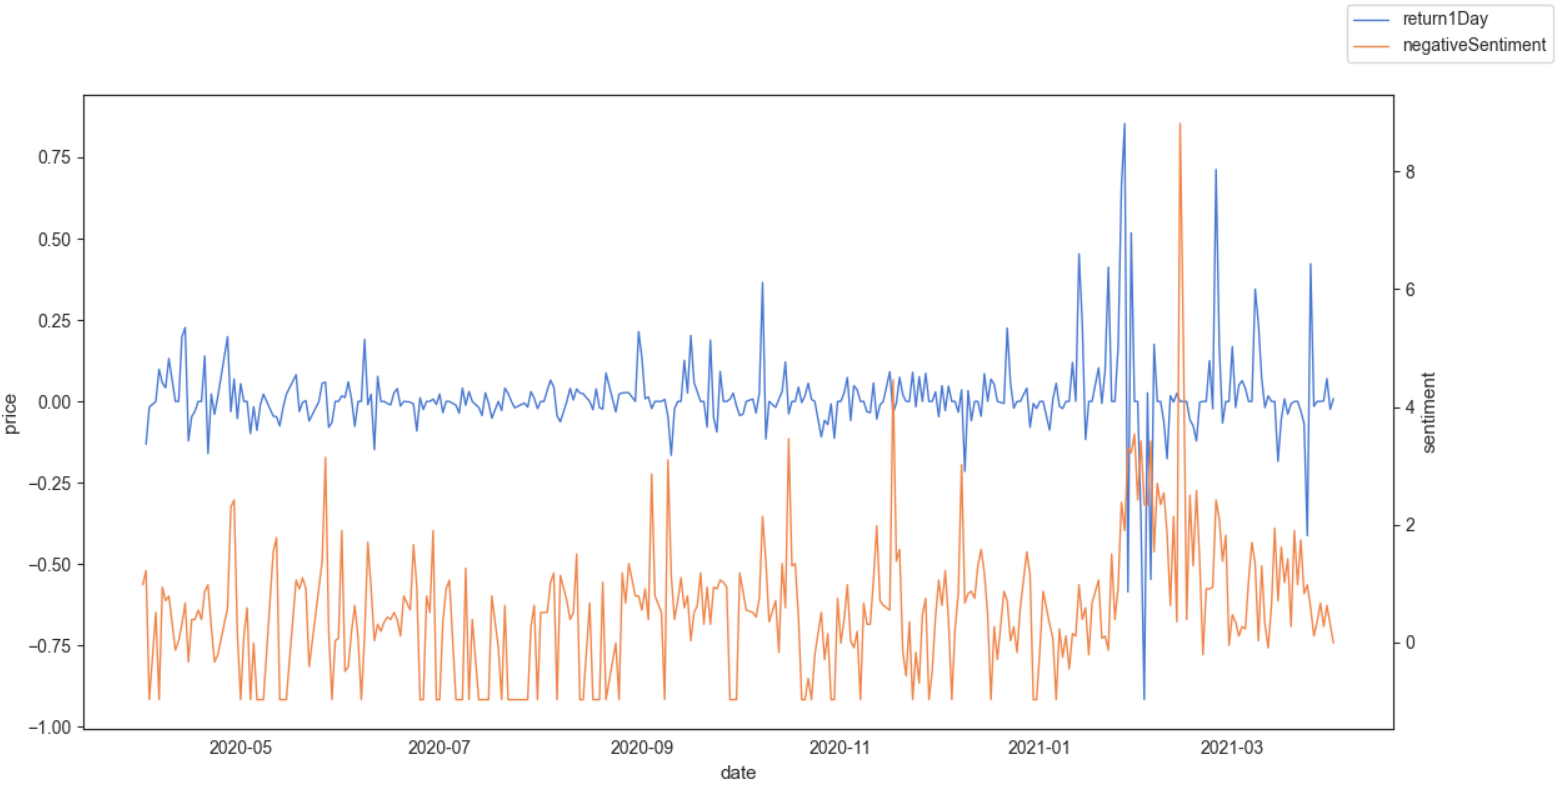
\includegraphics[width=15cm,height=10cm,keepaspectratio]{implementation/sampleGraph.png}
    \caption{Sample Graph}
    \label{fig:sampleGraph}
\end{figure}

\begin{lstlisting}[caption=Split Window into Multiple Subplots]
    fig, ax = plt.subplots()  
\end{lstlisting}
\begin{lstlisting}[caption=Create Overlapping Subplot]
    ax2 = ax.twinx()
\end{lstlisting}
\begin{lstlisting}[caption=Plot Dataset]
    ax.plot(dataset, color=colour, marker=marker, linewidth=linewidth) 
\end{lstlisting}
\begin{lstlisting}[caption=Plot Legend]
    fig.legend(legend)
\end{lstlisting}
\begin{lstlisting}[caption=Save picture of plot]
    fig.savefig('priceVsSentiment.jpg', format='jpeg', dpi=100, bbox_inches='tight')
\end{lstlisting}

\subsubsection{Single Point Estimator}

The Single Point Estimator can be broken down into 4 main steps:
\begin{enumerate}
    \item Create input and output series
    \item Input/Output Series Shuffling
    \item Model Testing
    \item Return Highest Accuracy Model and its accuracy
\end{enumerate}

\paragraph{Create input and output series}

The first step changes the prices and sentiment JSON object arrays into an array containing all of the desired columns, excluding date, as an array for each entry. As well as creating a second array with Boolean values for whether the next day's return is positive or negative. An example of this is if the close and volume columns are desired from the prices data-set and the negative sentiment column is desired from the sentiment data-set, the input series array elements would look like this \verb|[ closeValue, volumeValue, negativeSentimentValue ]|. If the next day's return for a given entry is positive, the output series element would be \verb|True|.

\paragraph{Input/Output Series Shuffling}

The shuffling simply randomises the order of the entries, so that there is no bias based on date. This is done using the function given by the \verb|sklearn.utils| module in the following way:
\begin{lstlisting}[caption=Shuffle series]
X, y = shuffle(X, y)
\end{lstlisting}
This function shuffles the order of both series while mainting the correspondece between the two sets.

\paragraph{Model Testing}

The model testing itself can be broken down into a discrete set of steps common accross all models. The difference being that some models require hyperparameter training, meanwhile others do not. These steps are:
\begin{itemize}
    \item \texttt{Hyperparameter Training} -- A hyperparameter is a parameter whose value is used to control the learning process, it is given as an input to the model. An example for a hyperparameter is the number of neighbors to examine for the \verb|KNeighborsClassifier|. Ranges of values are given and iterated through, the highest accuracy value is stored and used to create a final model.
    \item \texttt{K-Folds Cross-Validator} -- It provides train/test indices to split data in train/test sets. Split dataset into k consecutive folds (without shuffling by default). Each fold is then used once as a validation while the k - 1 remaining folds form the training set. This implementation uses 2 folds. This is an arbitrary value, further exploration may lead to finding a more suitable value. The \verb|kf.split(inputDataset)| is the function which excutes the split on the dataset.
    \begin{enumerate}
        \item \texttt{model.fit()} -- Train the model on the training dataset
        \item \texttt{model.predict()} -- Create a predicted output set given the test input dataset
        \item \texttt{accuracy\_score()} -- Calculate the accuracy of the values predicted from the model against the test output dataset
    \end{enumerate}
    \item \texttt{mean(kFoldAccuracies)} -- The mean accuracy of the accuracies calculated for each of the folds is set as the accuracy for the given hyperparameter
    \item \texttt{max(hyperparameterAccuracies)} -- The maximum accuracy of the accuracies calculated for the various hyperparameters is set as the defined accuracy for the model
    \item \texttt{timer} -- The \verb|perf_counter()| function from the \verb|time| module is used to time the training and discovery of hyperparameter for the model. The start time is set to before the iteration through the hyperparameters, and the end time is just after.
    \item \texttt{max(modelAccuracies)} -- The accuracy of the highest accuracy model as well as the trained model itself are returned
\end{itemize}
An example of the steps being executed on the KNeighborsClassifier is following:
\begin{lstlisting}[caption=KNeighborsClassifier Example]
kf = KFold(n_splits=2)

startTime = perf_counter()
K = range(1, 10)
highestAccuracyK = 0
highestKNNAccuracy = 0
for k in K:
    accuracies = []
    for train, test in kf.split(X):
        model = KNeighborsClassifier(n_neighbors=k).fit(X[train], y[train])
        pY = model.predict(X[test])
        accuracies.append(accuracy_score(y[test], pY))
    accuracies = np.array(accuracies)
    accuracy = np.mean(accuracies)
    if(accuracy > highestKNNAccuracy):
        highestKNNAccuracy = accuracy
        highestAccuracyK = k
print("Processed: ", model.__class__.__name__)
print("Time: ", round((perf_counter() - startTime) * 1000), "ms")
\end{lstlisting}

\paragraph{Accuracy Score vs Mean Squared Error}

An important point to discuss is the choice of function used in order to determine the accuracy of a given prediction set. The two options to consider are \verb|accuracy score| and \verb|mean squared error|. The \verb|accuracy score| option computes subset accuracy, the set of labels predicted for a sample must exactly match the corresponding set of correct labels. The \verb|mean squared error| of an estimator measures the average of the squares of the errors—that is, the average squared difference between the estimated values and the actual value. For this reason the choice when using classifier models is the \verb|accuracy score| option since classifier results are either labelled correctly or not.

\paragraph{Models Comparison}

For this component a number of models are used in order to find the most accurate model for a given dataset. The following models were all chosen because they are various different different models which are excellent at classifications. They each have different strength and weaknesses, and for that reason one the models may work better or worse depending on the dataset.
\begin{itemize}
    \item \texttt{KNeighborsClassifier (KNN)} -- KNN is a non-parametric and lazy learning algorithm. Non-parametric means there is no assumption for underlying data distribution. In KNN, K is the number of nearest neighbors. The number of neighbors is the core deciding factor. What this means is that the decision for the output will be based on the k nearest neightbors. K is determined through hyperparameter training as described above.
    \begin{figure}[h]
        \centering
        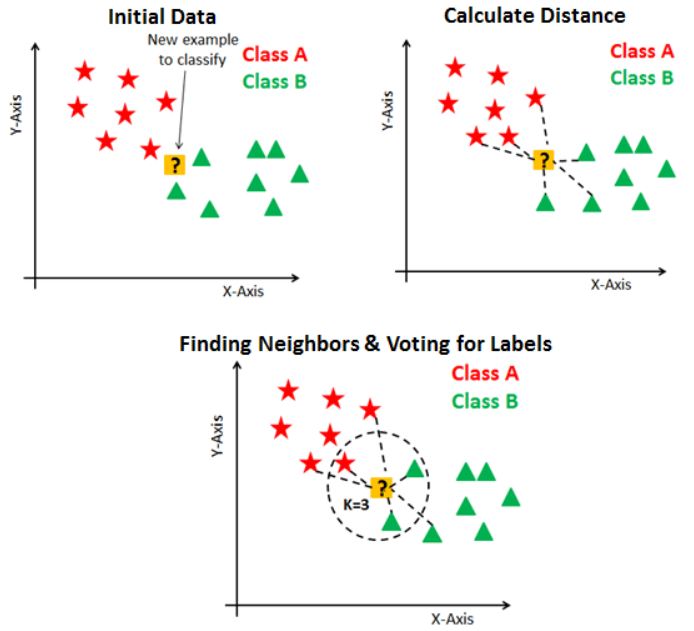
\includegraphics[width=15cm,height=5cm,keepaspectratio]{implementation/kNN.png}
        \caption{KNeighborsClassifier}
        \label{fig:kNN}
    \end{figure}
    \item \texttt{DecisionTreeClassifier} -- A decision tree is created from the training data in order to achieve the classification. A decision tree is a flowchart-like tree structure where an internal node represents a feature, the branch represents a decision rule, and each leaf node represents the outcome. This can be seen in the figure below.
    \begin{figure}[h]
        \centering
        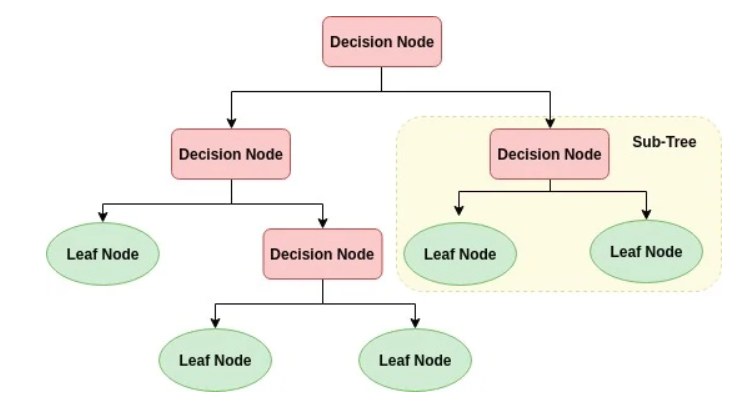
\includegraphics[width=15cm,height=5cm,keepaspectratio]{implementation/decisionTree.png}
        \caption{Decision Tree}
        \label{fig:decisionTree}
    \end{figure}
    Within the system the \verb|DecisionTreeClassifier()| class is created. However to quickly cover the steps in creating a decision tree, they are the following:
    \begin{enumerate}
        \item Select the best feature using Attribute Selection Measures to split the dataset. Attribute selection measure is a heuristic for selecting the splitting criterion that partition data into the best possible manner. Attribute Selection Measure provides a rank to each feature by explaining the given dataset. There are multiple ways of assigning each feature a value. Some of these being:
        \begin{itemize}
            \item \texttt{Information Gain} -- It computes the difference between entropy before split and average entropy after split of the dataset based on given attribute values
            \item \texttt{Gain Ratio} -- It extends Information Gain by handling the issue of bias by normalizing the information gain using Split Info
        \end{itemize}
        \item Make that feature a decision node and breaks the dataset into smaller subsets.
        \item Starts tree building by repeating this process recursively for each child until one of the condition will match:
        \begin{itemize}
            \item All the tuples belong to the same feature value.
            \item There are no more remaining features.
            \item There are no more instances.
        \end{itemize}
    \end{enumerate}
    \item \texttt{GaussianProcessClassifier} -- It is a classifier which uses Gaussian Processes. Gaussian Processes are a generalization of the Gaussian probability distribution. They are a type of kernel model capable of predicting highly calibrated class membership probabilities, although the choice and configuration of the kernel used at the heart of the method can be challenging. For the purposes of this project an arbitrarily chosen kernel configuration was chosen in order to simplify the process. The choice was the basic confugration shown in the documentation for the class. A radial basis function was used to create this.  A radial basis function being a real-valued function whose value depends only on the distance between the input and some fixed point. For further explanation, the documentation for this can be referenced.
    \item \texttt{AdaBoostClassifier} -- AdaBoost or Adaptive Boosting is a type of ensemble boosting classifier. Boosting algorithms are a set of weak classifiers which create a strong classifier. These algorithms help decrease model bias. The basic concept behind Adaboost is to set the weights of classifiers and training the data sample in each iteration such that it ensures the accurate predictions of unusual observations. The general steps for this classifier are:
    \begin{enumerate}
        \item Initially, all observations are given equal weights
        \item A model is built on a subset of data
        \item Using this model, predictions are made on the whole dataset
        \item Errors are calculated by comparing the predictions and actual values
        \item While creating the next model, higher weights are given to the data points which were predicted incorrectly
        \item Weights can be determined using the error value. For instance, the higher the error the more is the weight assigned to the observation
        \item This process is repeated until the error function does not change, or the maximum limit of the number of estimators is reached
    \end{enumerate}
    \item \texttt{RandomForestClassifier} -- This algorithm creates decision trees on randomly selected data samples, gets a prediction from each tree and selects the best solution by means of voting. The n hyper parameter must be trained, this determines the number of forests to use, i.e. the number of random samples. The general steps are:
    \begin{enumerate}
        \item Select random samples from a given dataset
        \item Construct a decision tree for each sample and get a prediction result from each decision tree
        \item Perform a vote for each predicted result
        \item Select the prediction result with the most votes as the final prediction
    \end{enumerate}
    \begin{figure}[h]
        \centering
        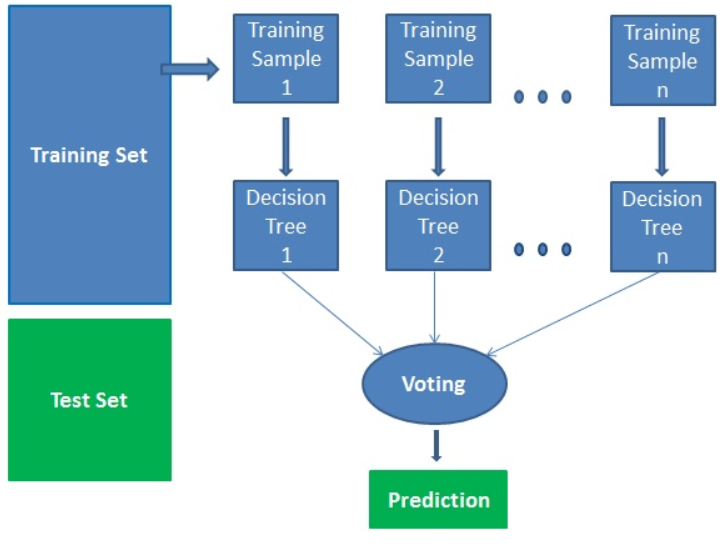
\includegraphics[width=15cm,height=7cm,keepaspectratio]{implementation/randomForest.png}
        \caption{RandomForestClassifier}
        \label{fig:randomForest}
    \end{figure}
\end{itemize}

\paragraph{Return Highest Accuracy Model and its accuracy}

The accuracy of the different models is compared and the highest accuracy model is returned to the user.

\subsubsection{Autocorrelator}

The menu for the autocorrelator allows the selection of a column and lag to be examined. This component calculate the correlation between a column and itself with an offset of n days. N starts at 1 and calculates the autocorrelation for every integer until the lag amount is reached. All of these values are returned.

\begin{lstlisting}[caption=Example AutoCorrelator Output when lag = 5 for return1Day column]
return1Day Auto Correlation
1 day lag 0.010044065231783677
2 day lag 0.13420635746867923
3 day lag 0.17706335839486953
4 day lag -0.23281554097728582
5 day lag 0.0305722042951903
\end{lstlisting}

The way correlation is calculated is using linear regression. The \verb|scipy.stats| module provides a function, \verb|linregress()|, which allows this. The \verb|rvalue| extracted from the output is the correlation coefficient. The \verb|rvalue|, the coefficient of determination, is the proportion of the variance in the dependent variable that is predictable from the independent variable, i.e. correlation.

\subsubsection{Return Vs Sentiment Correlator}

This component is strict in its use. It calculates the correlation between return1Day and negativeSentiment at preset lags. These being same day and 1 day lag, with return1Day one day and negativeSentiment the next day and viceversa. Correlation is calculated in the same way as within the AutoCorrelator, i.e. using linear regression.

\begin{lstlisting}[caption=Example Return Vs Sentiment Output]
return1Day/negativeSentiment Correlation
same day -0.009080953348214611
1 day lag return1Day to negativeSentiment 0.060205743120825606
1 day lag negativeSentiment to return1Day -0.052446888115240176
\end{lstlisting}

\subsubsection{Descriptive Statistics}

The menu for this component allows for the selection of the desired column. It the calculates the descriptive statistics for the column. It also displays a graph in order to allow for a better understanding of the statistics. The descriptive statistics shown are:
\begin{itemize}
    \item \texttt{Mean} -- The average of all the data-points
    \item \texttt{Standard Error} -- Measures the accuracy with which a sample distribution represents a population by using standard deviation
    \item \texttt{Median} -- The value separating the higher half from the lower half of a data-set
    \item \texttt{Mode} -- The most common value in the data-set
    \item \texttt{Standard Deviation} -- Measures the amount of variation or dispersion of the data-points
    \item \texttt{Sample Variance} -- The average of the squared differences from the mean, helps measure variance within the data-points
    \item \texttt{Kurtosis} -- Defines how heavily the tails of a distribution differ from the tails of a normal distribution, i.e. it measures the number of extreme values in the data-set
    \item \texttt{Skewness} -- Measures the asymmetry of the distribution about its mean
    \item \texttt{Range} -- The difference between the maxim and minimum values
    \item \texttt{Minimum} -- The minimum value found in the data-points
    \item \texttt{Maximum} -- The maximum value found in the data-points
    \item \texttt{Sum} -- The sum of the data-points
    \item \texttt{Count} -- The number of data-points analysed
\end{itemize}

\begin{figure}[h]
    \centering
    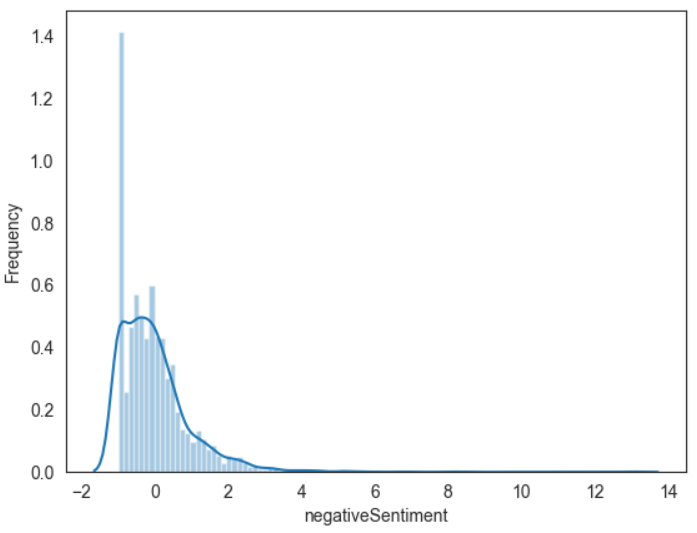
\includegraphics[width=15cm,height=9cm,keepaspectratio]{implementation/descriptiveGraph.png}
    \caption{descriptiveGraph}
    \label{fig:descriptiveGraph}
\end{figure}

\subsubsection{Vector Autoregressor}

For this section, the Gretl software was used to gather the desired results. The steps to using Gretl for Vector Autoregression analysis are the following:
\begin{enumerate}
    \item Use an excel sheet created by the python program
    \item Import excel sheet into gretl
    \item Change the data to have a time-series interpretation
    \item Select the desired VAR multi-variate model, this analysis used the base Vector Autoregression model
    \item Add the desired endogeneous and exogenous variables
    \item Analyse the values returned
\end{enumerate}

\section{Implementation Summary}

In this chapter, the technologies used and how they were used to implement the design decided upon is discussed. It breaks down specifics of implementation as well as discussing why certain choices were made within.